\documentclass[../analisi.tex]{subfiles}
\graphicspath{{\subfix{../pics/}}}
\begin{document}

\section{Funzioni}
\subsection{Introduzione}

\begin{defn}
Una funzione $f$ é una relazione tra gli elementi di due insieme $A$ e $B$ che ad ogni elemento di \bt{A} associa \bt{uno ed un solo} elemento di \bt{B}.
\end{defn}


Una funzione è definita assegnando:
\begin{itemize}
\item un insieme \tit{A} detto  \textsc{dominio}
\item un insieme \tit{B} detto \textsc{codominio}
\item una relazione $f: A \rightarrow B$ che associa ogni elemento di A uno ed un solo elemento di B
\end{itemize}


\subsection{Tipi di funzioni}

Una funzione $f(x)$ può essere di 3 tipi:
\begin{enumerate}
    \item \bt{suriettiva}
    \item \bt{iniettiva}
    \item \bt{biiettiva} se è \underline{sia} \bt{iniettiva} e  \bt{suriettiva}
    \end{enumerate}

    \begin{defn} Una funzione si dice \bt{iniettiva} quando ad elementi \bt{distinti} del \normalfont{\textsc{dominio}} corrispondono elementi \bt{distinti} del \normalfont{\textsc{codominio}}
\begin{equation}
  f(a_1) = f(a_2) \Rightarrow a_1 = a_2
\end{equation}

\begin{figure}[ht]
	\center
	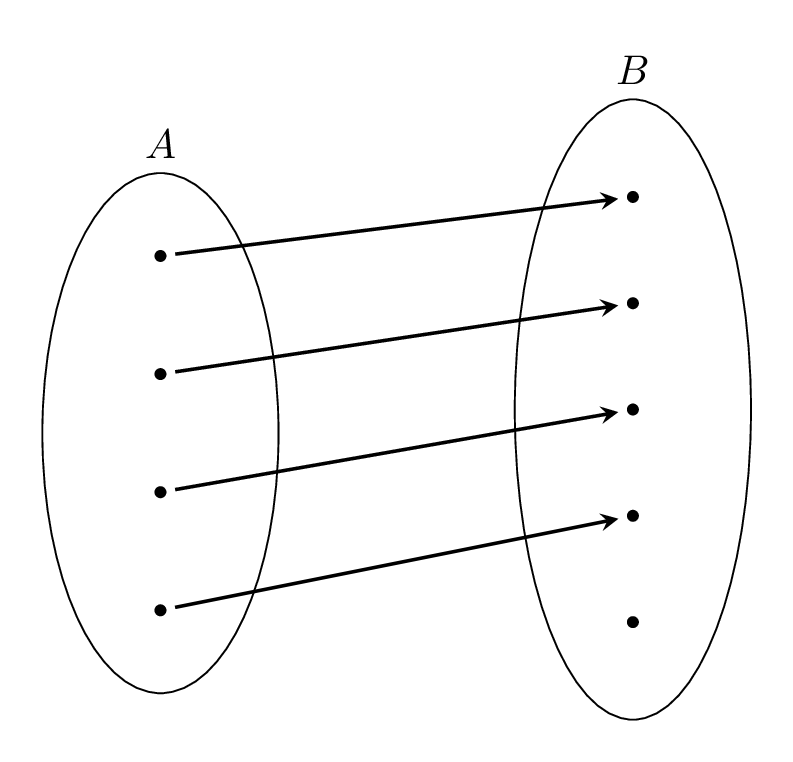
\includegraphics[scale=0.135]{iniettiva}
	\caption{grafico iniettiva}
	\label{fig:grafico_iniettiva}
\end{figure}
\end{defn}
\noindent


\begin{defn} Una funzione si dice \bt{suriettiva} qunado \bt{ogni} elemento del codominio è immagine di \bt{almeno} un elemento del dominio.
\begin{equation}
  b\in B \rightarrow \exists a \in A : f(a) = b
\end{equation}

\begin{figure}[ht]
	\center
	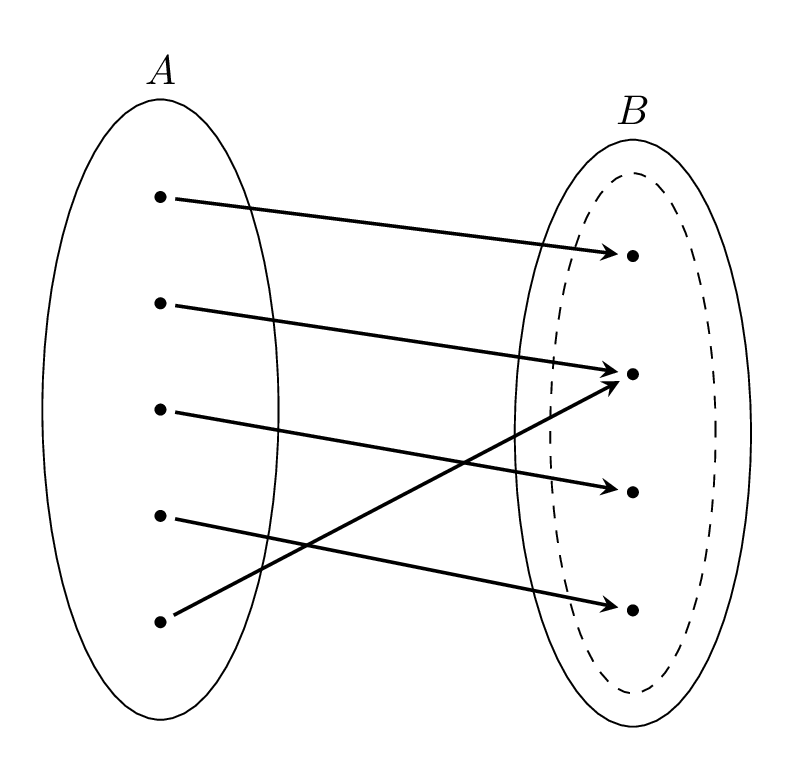
\includegraphics[scale=0.15]{suriettiva}
	\label{fig:grafico_suriettiva}
	\caption{graifco suriettiva}
\end{figure}
\end{defn}


\begin{eser}
Dimostra di che tipo è questa funzione:\vspace{1.5mm}

\begin{equation}
  f :\R\rightarrow \R \qquad f(x)=x^2
\end{equation}

\end{eser}

\begin{dimo}
Non può essere iniettiva perchè per ogni numero reale positivo ne esiste uno uguale negativo, il cui qudrato sarà il \bt{medesimo}.\vspace{1.5mm}

\begin{equation}
  se\quad x_1 = -x_2 \quad \Rightarrow \quad f(x_1) = f(x_2)
\end{equation}  

\vspace{2mm}
si può provare inoltre che non è una funzione suriettva in quanto \bt{nessun} numero negativo fa parte del codominio ed esso è formato da $\R$ dunque
\begin{equation}
  -4 \ne f(x) \qquad \forall x \in \R
\end{equation}
\end{dimo}

\begin{eser}
Dimostra di che tipo è questa funzione:
\begin{equation}
  f :\N\rightarrow \N \qquad f(x)=x^2
\end{equation}
\end{eser}

\begin{dimo}
  se cambiamo il dominio e il codominio nell'insieme dei numeri naturali e consideriamo la stessa legge possiamo deddure che:

\begin{equation}
  \forall n,m : n \ne m \quad \Rightarrow \quad n^2 \ne m^2
\end{equation}

\vspace{3.5mm}
Per \bt{qualsiasi} coppia di numeri naturali diversi fra loro non è possibile pensare che il loro quadrato sia uguale, per tanto la funzione è iniettiva. 
\vspace{2.5mm}
Inoltre \bt{qualsiasi} numero dispari non avrà una propria immagine, in quanto l'insieme racchiude \bt{solo} numeri interi positivi. Ovvero:

\begin{equation}
  \exists \frac{x}{2} \in \N: \{y = x + 1\} \quad
  \Rightarrow \quad y \ne n^2 \qquad \forall n\in \N
\end{equation}

\end{dimo}


\subsection{Funzioni invertibili}
\begin{defn} Una funzione $f:A\rightarrow B$ si dice invertibile se esiste una funzione $g: B \rightarrow A$ chiamata funzione inversa tale che:
\begin{itemize}
  \item $\forall a\in A, \quad g(f(a))=a$
  \item $\forall b\in B, \quad f(g(b))=b$
\end{itemize}
Essa si può considerare invertibile se è \bt{biiettiva}.
\end{defn}

\begin{eser}
  Dimostra se la funzione $f: \R \ \rightarrow \ \R \qquad f(x) = 2x\ +\ 1$ è inversibile.
\end{eser}

\begin{dimo}
Ponendo l'equazione $ y =\ 2x\ +\ 1$ deduciamo che

	\begin{equation}
  		f^{(-1)}(x) = \frac{x\ -\ 1}{2}
	\end{equation}

\vspace{1.5mm}
quindi:
\begin{equation}
  f^{(-1)}(f(x))= f^{(-1)}(2x\ +\ 1)\ = \frac{(2x\ +\ 1)\ -\ 1}{2}\ =\ x;
\end{equation}
\vspace{1.5mm}
e allo stesso tempo

\vspace{1.5mm}
\begin{equation}
f(f^{(-1)}(y))\ = f(\frac{y\ -\ 1}{2})\ +\ 1\ =\ y
\end{equation}
\end{dimo}

\subsection{Piano Cartesiano}
Fissando un'origine e un'unità di misura ad \bt{ogni} punto di una retta orientata corrisponde uno ed un solo numero reale.
Si stabilisce così una \bt{corrispondenza biunivoca} tra i punti della retta orientata e i numeri reali.\\
Data la funzione
\vspace{1.5mm}

\begin{equation}
  f: A\ \rightarrow\ B \quad A,B\ \subseteq \R\ \times\ \R\ = \R^2\\
\end{equation}

\begin{figure}[ht]
  \center
  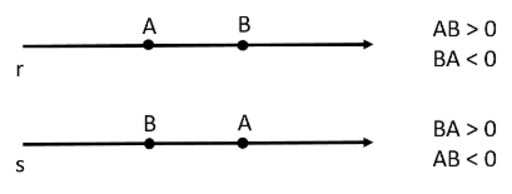
\includegraphics[scale=0.25]{rettaorientata}
  \caption{la retta orientata}
  \label{fig:retta_orientata}
\end{figure}

\begin{defn}
Definiamo una \bt{coppia} di rette orientate disposte \bt{perpendicolarmente} fra loro \bt{assi coordinati}.
\begin{itemize}
  \item{La retta da destra verso sinistra viene chiamata \bt{asse delle ascisse}}
  \item{la retta dal basso verso l'alto viene chiamata \bt{asse delle ordinate}}
\end{itemize}
Il punto del piano in cui si incontrano viene chiamato \bt{origine degli assi} e viene indicato con $O$
\end{defn}

Un qualsiasi punto del piano $P$ viene identificato con una ascissa $x_p$ ed una ordinata $y_p$, quindi $P(x_p, y_p)$.\\
Il piano viene diviso in IV quadranti numerati in senso antiorario.

\begin{figure}[ht]
  \center
  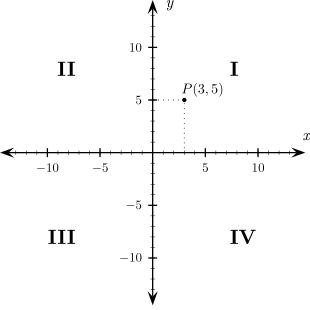
\includegraphics[scale=0.4]{pianocartesiano}
  \caption{il piano cartesiano}
  \label{fig:piano_cartesiano}
\end{figure}

\subsection{Grafici di funzioni}
\raggedright{Ora possiamo rappresentare graficamente coppie ordinate di numeri reali sul piano, quindi possiamo rappresentare il \bt{grafico} di una funzione}

\begin{equation}
f: A\ \subseteq \R\  \rightarrow \ B \subseteq \R\
\end{equation}\\ \vspace{1.5mm}

e tutte le coppie $(x,\ f(x))$ tali che $x\in A$:\\

\begin{equation}
G(f)\ = \{(x,\ f(x))\} \ :\ x\in A
\end{equation}

\begin{figure}[ht]
  \center
  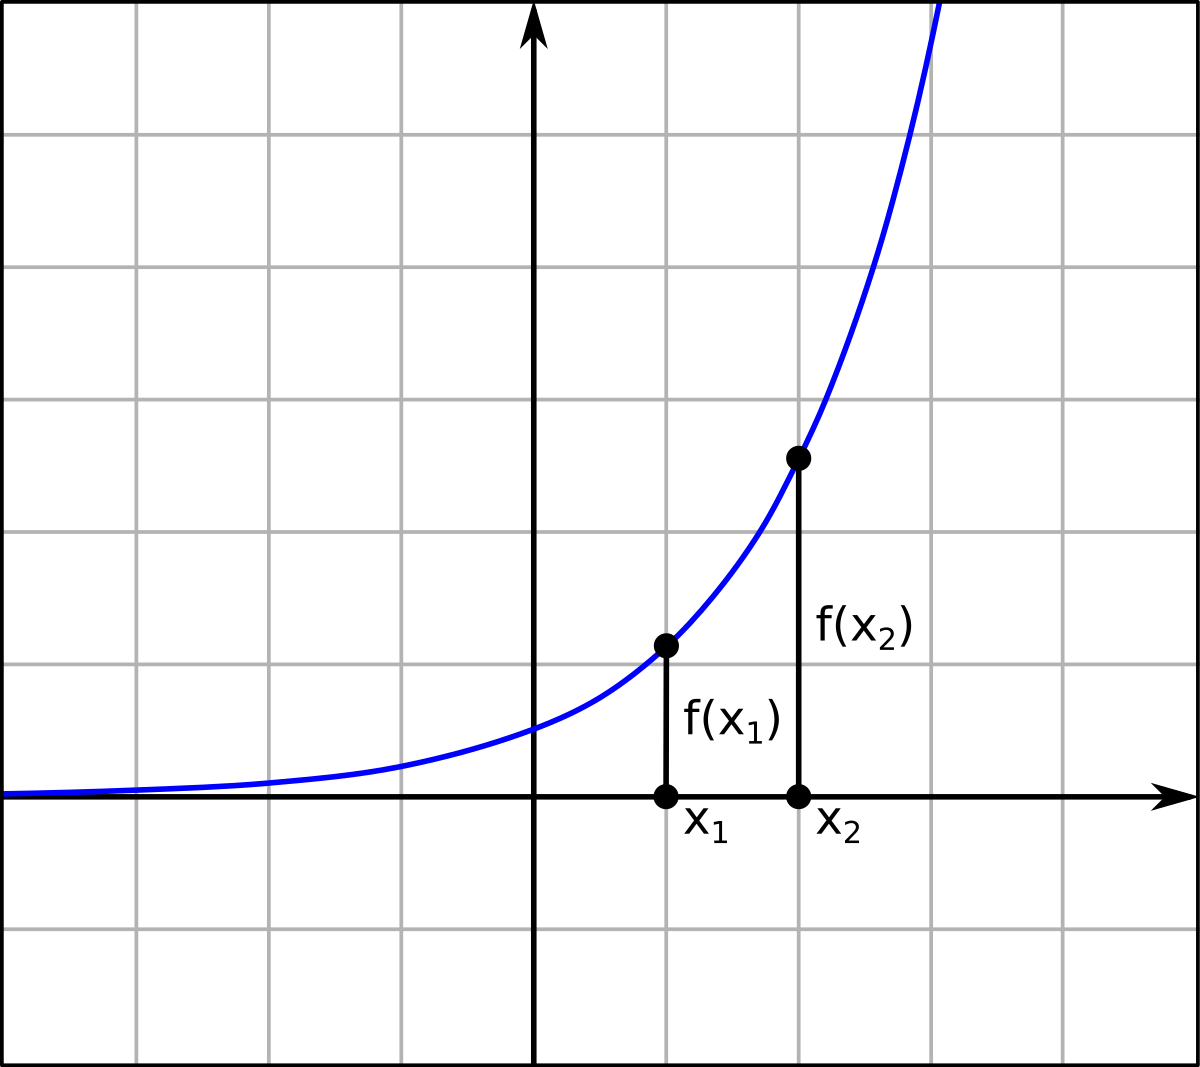
\includegraphics[scale=0.15]{graficofunzione}
  \caption {il grafico di una funzione crescente}
  \label{fig:grafico_funzione}
\end{figure}

\subsection{Funzioni Pari e Dispari}
\begin{defn}
Una funzione $f: [-a, a]\ \rightarrow \ \R$ si dice \bt{pari} se $f(x) = f(-x)$\\
Si deduce quindi che il grafico di una funzione così definita è simettrico rispetto all'\bt{asse delle ordinate}
\end{defn}

\begin{figure}
  \center
  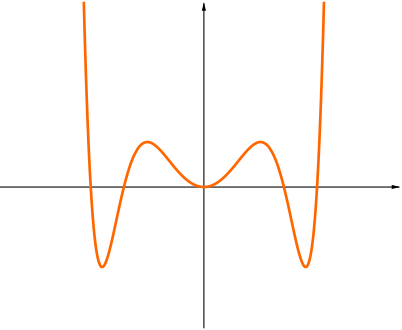
\includegraphics[scale=0.65]{funzionepari}
  \caption{Una funzione pari}
  \label{fig:funzione_pari_grafico}
\end{figure}


\begin{defn}
Una funzione $f: [-a, a]\ \rightarrow \ \R$ si dice \bt{dispari} se $f(-x) = -f(x)$\\
Si deduce quindi che il grafico di una funzione così definita viene \bt{specchiata} in due quadranti uno \bt{oppsoto} all'altro
\end{defn}

\begin{figure}[ht]
  \center
  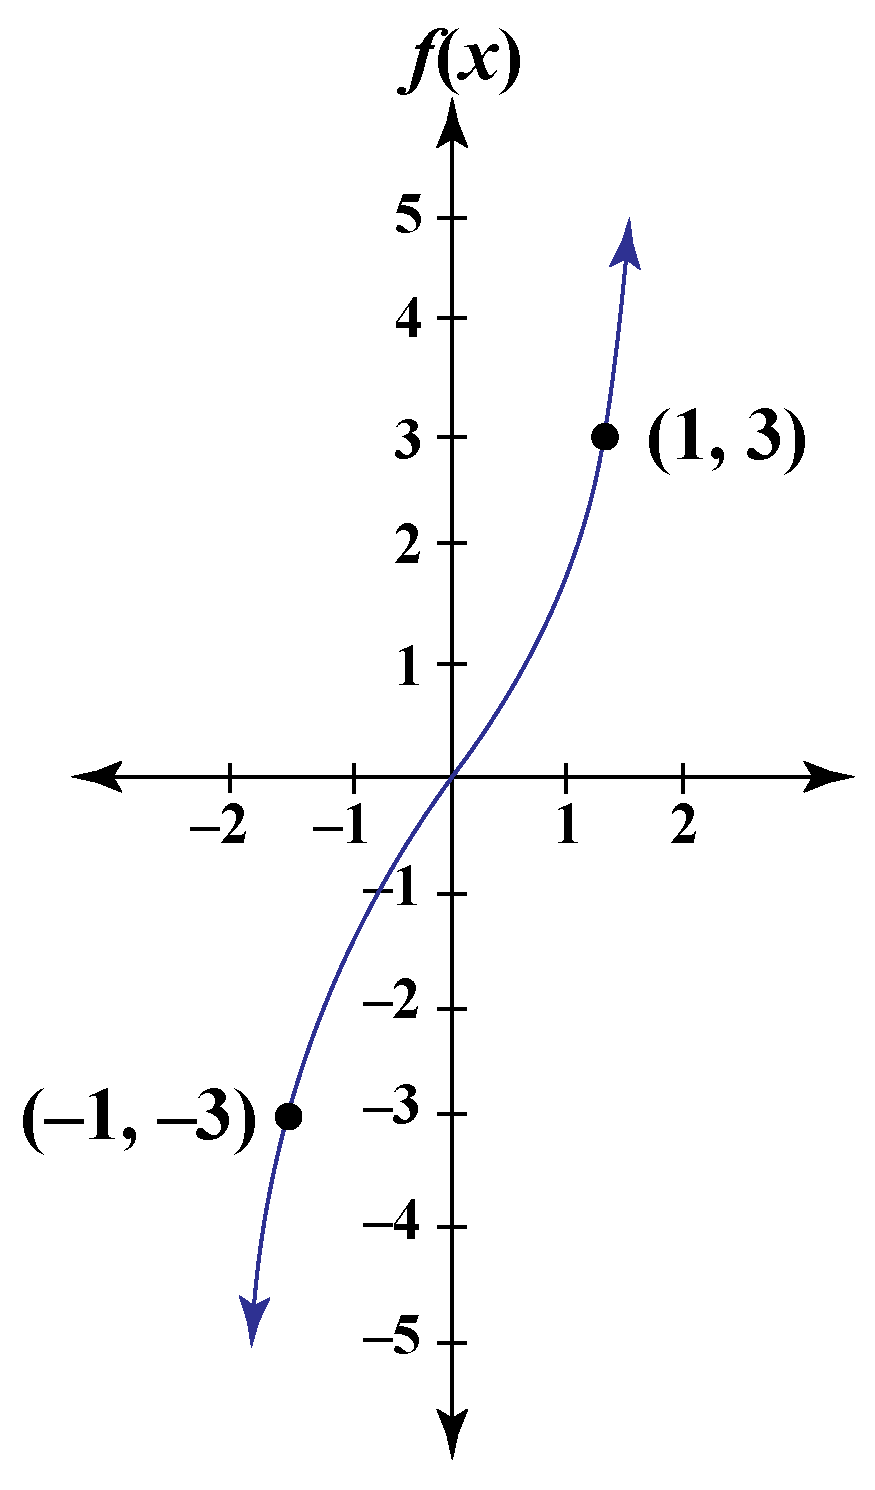
\includegraphics[scale=0.25]{funzionedispari}
  \caption{Una funzione dispari}
  \label{fig:funzione_dispari_grafico}
\end{figure}



\subsection{Funzioni crescenti e decrescenti}
\begin{defn}
 Una funzione $f: [-a, a]\ \rightarrow \ \R$ si dice \bt{crescente} se
 \begin{equation}
   f(x_2)\ \geq \ f(x_1) \quad \forall x_2 > x_1 \in [a,b]
\end{equation}\\
 Si dice \bt{strettamente crescente} se\\
 \begin{equation}
  f(x_2)\ \>\ f(x_1) \quad \forall x_2 > x_1 \in [a,b]
\end {equation}


\begin{figure}[ht]
  \center
  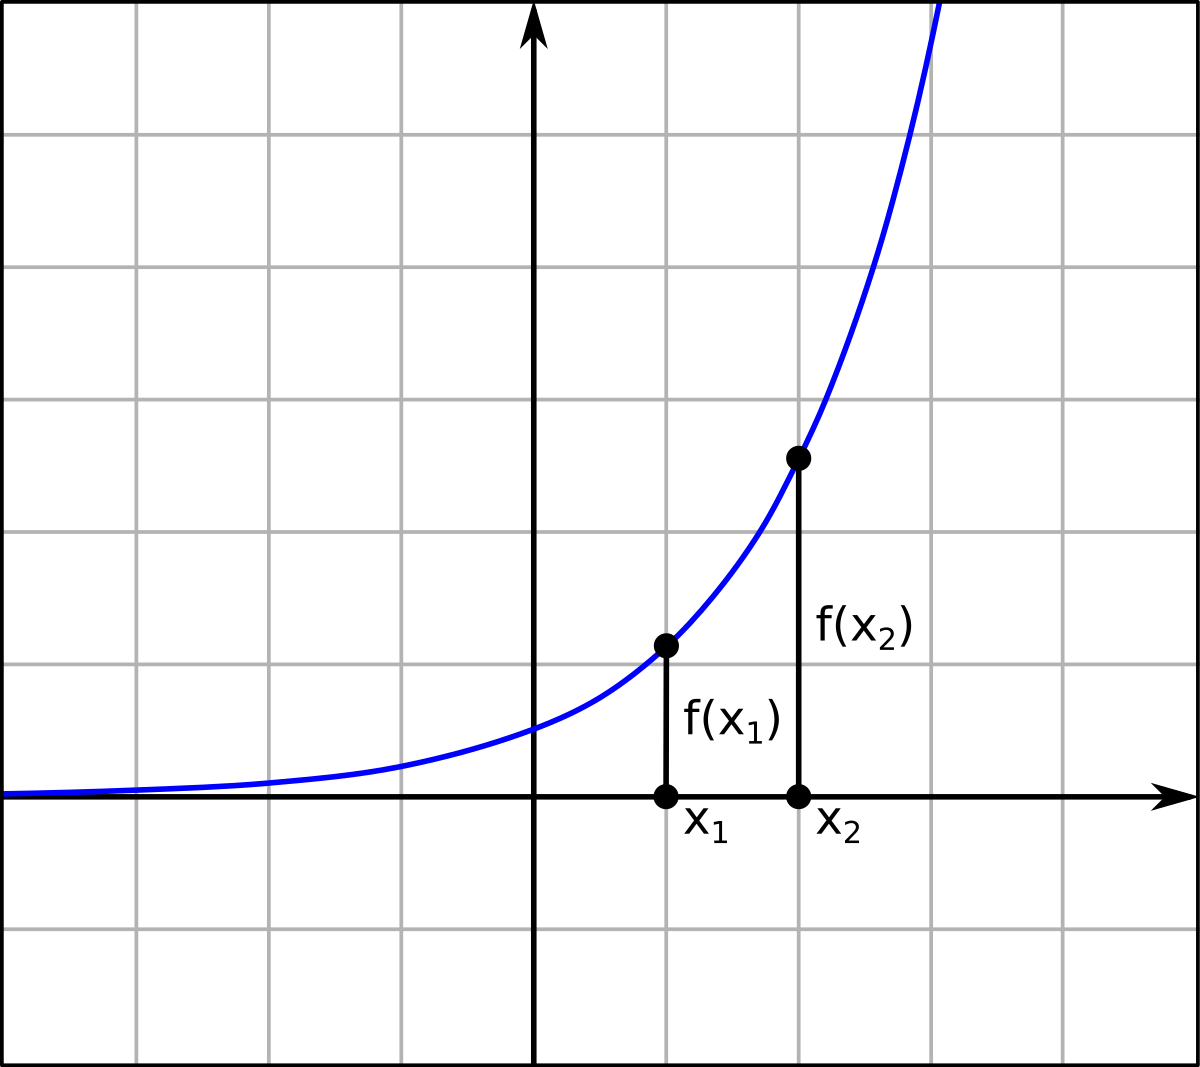
\includegraphics[scale=0.15]{graficofunzione}
  \caption {il grafico di una funzione crescente}
  \label{fig:grafico_funzione_crescente}
\end{figure}

\end{defn}



\begin{defn}
 Una funzione $f: [-a, a]\ \rightarrow \ \R$ si dice \bt{decrescente} se
 \begin{equation}
   f(x_2)\ \leq \ f(x_1) \quad \forall x_2 > x_1 \in [a,b]
\end{equation}\\
 Si dice \bt{strettamente decrescente} se\\
 \begin{equation}
  f(x_2)\ <\ f(x_1) \quad \forall x_2 > x_1 \in [a,b]
\end{equation}


\begin{figure}[ht]
  \center
  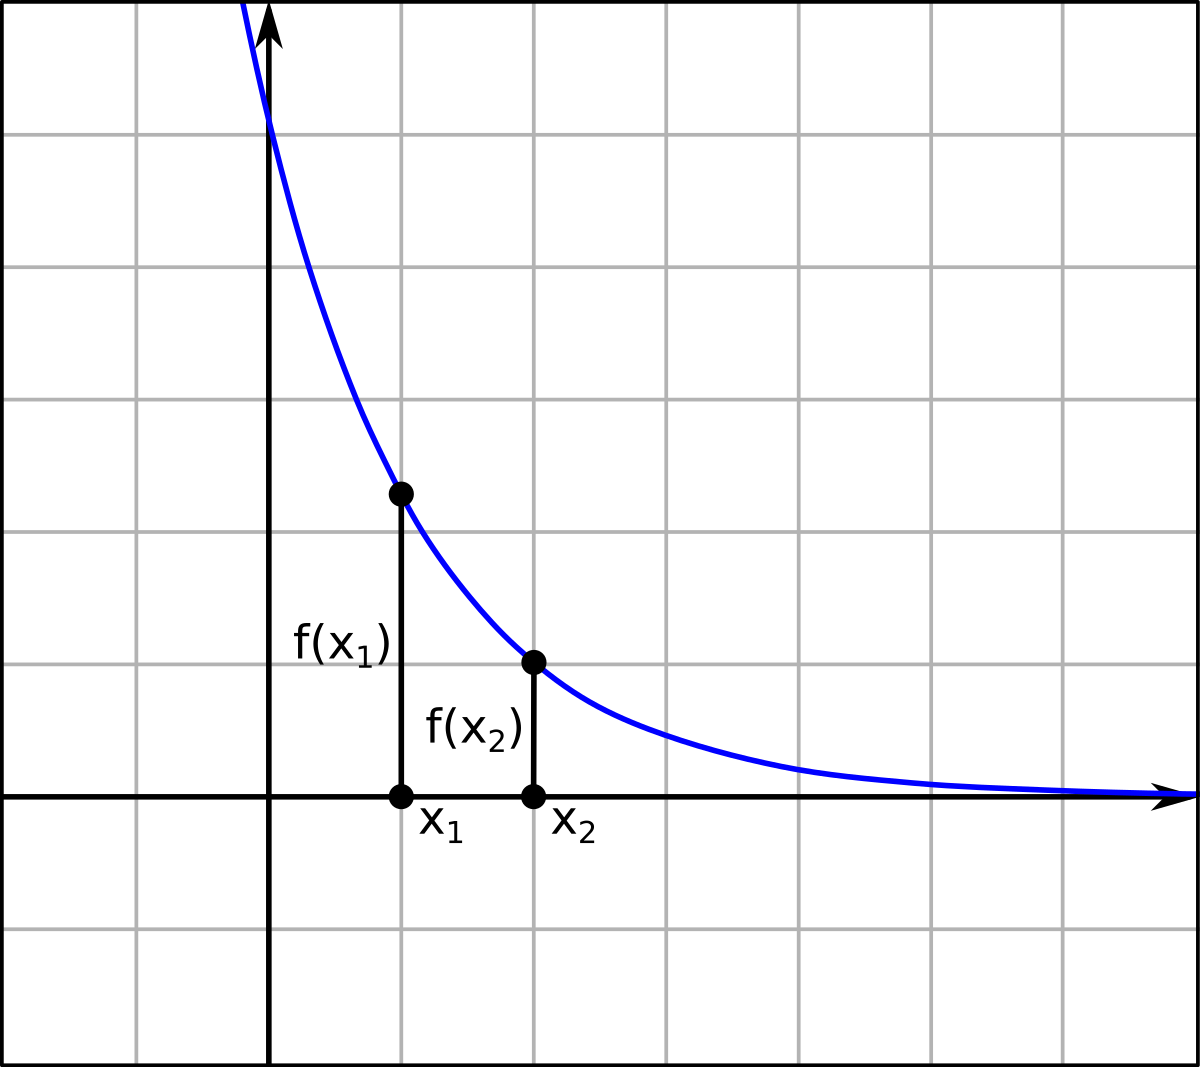
\includegraphics[scale=0.15]{funzionedecrescente}
  \caption {il grafico di una funzione decrescente}
  \label{fig:grafico_funzione_decrescente}
\end{figure}

\end{defn}

\subsection{Funzioni inverse}
Se i punti di una funzione $ f : A\ \rightarrow \ B \quad A,B \subseteq \R $ si ottengono dalle coppie $ (a,b)\in A\ \times\ B $
\begin{defn}
Il grafico di una funzione inversa si ottiene invertendo le coordinate dei punti del grafico. Ovvero i punti del grafico della \bt{funzione inversa} si ottengono dalle coppie $(b,a)\ \in B\ \times\ A\ $ //
Per via grafica esso può essere ottenuto \bt{riflettendo} il grafico rispetto alla \bt{bisettrice} del \bt{primo} e \bt{terzo quadrante}

\begin{figure}[ht]
  \centering
  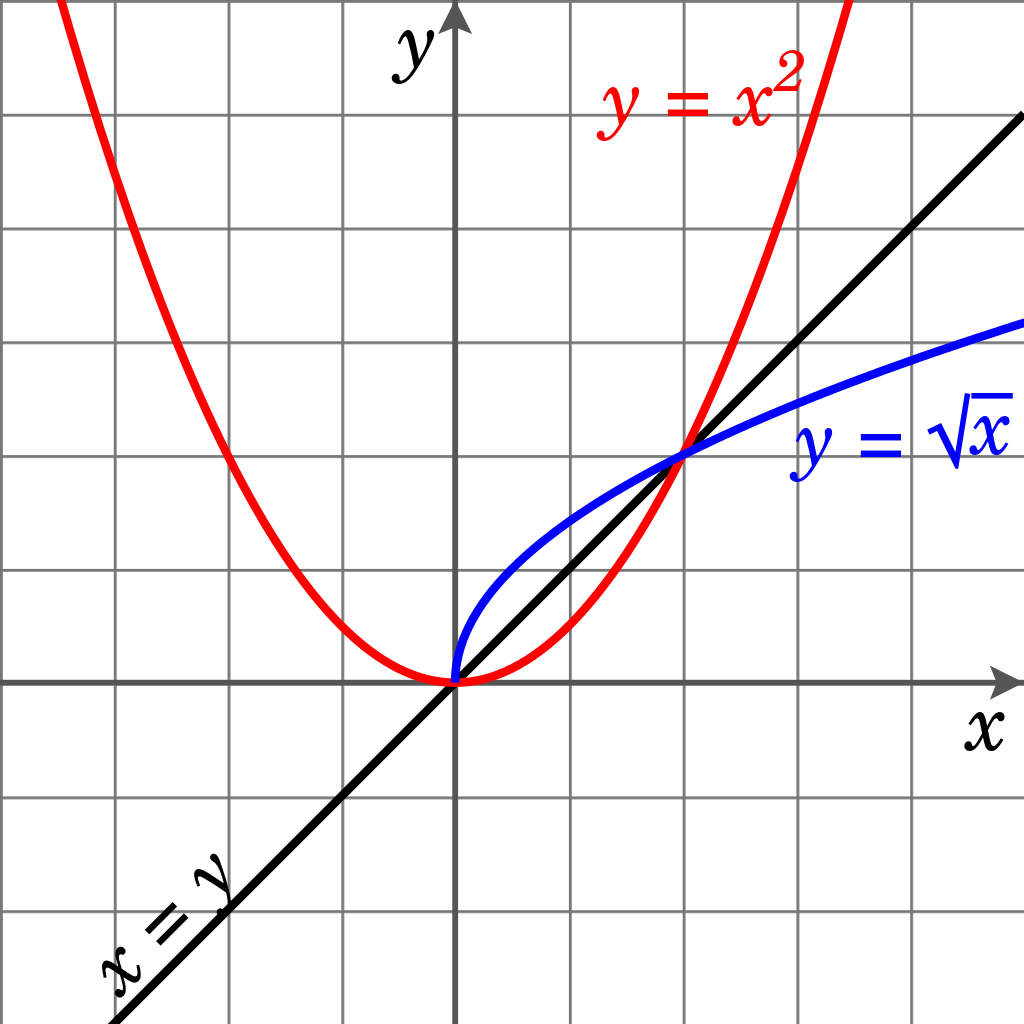
\includegraphics[scale=0.1]{funzioneinversa}
  \caption{Il grafico di una funzione inversa}
  \label{fig:grafico_funzione_inversa}
\end{figure}
\end{defn}

% end of first unit


\subsection{Modelizzazione matematica}

\begin{defn}
  Per \bt{modelizzazione matematica} si intende un porcesso che ha per scopo quello di \bt{interpretare} fenomeni legati al mondo reale partendo da dati sperimentali e \bt{traducendoli} in \bt{problemi matematici}\\
\end{defn}

Per passare da un fenomeno reale alla sua descrizione mediante modello matematico è necessario un processo di \bt{astrazione} e \bt{traduzione} del fenomeno in termini matematici e rigorosi. \\

\vspace{1mm}
Quando si vuole modelizzare un certo fenomeno, si vuole capire \bt{come} le variabili coinvolte siano in relazione tra loro, ovvero stabilire delle \bt{leggi matematiche} che descrivono queste relazioni. \\

\vspace{1mm}
La procedura di modelizzazione è:
\begin{enumerate}
  \item si identifica l'incognita del problema
  \item si analizza il fenomeno fisico e si raccolgono informazioni
  \item si individuano le relazioni tra le informazioni raccolte, che poi vengono tradotte in equazioni
  \item si risolvono le equazioni ottenute e se ne verifica la validità del modello
\end{enumerate}


In un modello matematico che coinvolge due grandezze x ed y ci interessa capire come la \bt{variabile dipendente $(y)$} varia al variare di quella \bt{indipendente}\\

\begin{esem}
Supponiamo di aver formulato la legge $ y\ =\ f(x)\ $\\
Se il modello è giusto potremmo ricavare il valore di $y$ a partire da qualsiasi valore di $x$ senza effettuare ulteriori esperimenti e misurazioni.\\
Rappresentandolo graficamente:

\begin{figure}[ht]
  \center
  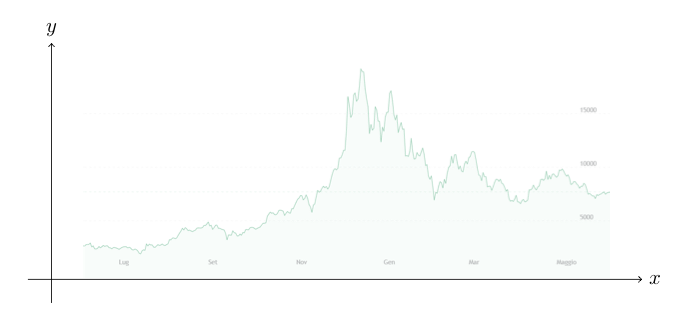
\includegraphics[scale=0.75]{graficobitcoin}
  \caption{Il grafico dell'andamento dei bitcoin}
  \label{fig:btc_chart}
\end{figure}
Questo è il grafico di $y\ =\ f(x)$ dove y="valore del bitcoin in dollari" e x="tempo".
\end{esem}

\subsection{Proporzioni}
\begin{defn}
  Due grandezze $A$ e $B$ si dicono \bt{direttamente proprozionali} se esiste un numero $c$ detto \bt{costante di proporzionalità} tale che:

\begin{equation}
  A\ =\ cB
\end{equation}
\end{defn}

Questo significa che le due grandezze sono legate da una certa legge, per la quale quando una raddoppia, triplica, dimezza, di conseguenza la seconda raddoppia, triplica, dimezza etc.

\begin{esem}
  $A$ = "quantità di chilometri che l'auto può percorrere"\\
  $B$ = "litri di carburante nel serbatoio"
\end{esem}

\begin{defn}
  Due grandezze $A$ e $B$ si dicono \bt{inversamente proprozionali} se esiste un numero $c$ detto \bt{costante di proporzionalità} tale che:

\begin{equation}
  AB\ =\ c
\end{equation}
\end{defn}
Questo significa che le due grandezze sono tali che all'aumentare di una, l'altra diminuisce proporzionalmente.

\begin{esem}
  $A$ = "numero di partecipanti all'acquisto di un immobile"\\
  $B$ = "quota per partecipante"\\
  $c$ = costo dell'immobile
\end{esem}

\end{document}
